\documentclass[a4paper,12pt]{article}
%\documentclass[a4paper,12pt,twoside]{book}

\usepackage[margin=3.5cm]{geometry}

\usepackage[utf8x]{inputenc}
\usepackage[ngerman]{babel}
\usepackage{longtable}
\usepackage{amsmath}
\usepackage{amsfonts}
\usepackage{amssymb}
\usepackage{amsthm}
\usepackage{graphicx}
\usepackage{tikz}
\usepackage{epsfig}
%\usepackage[utf-8]{inputenc}
\usepackage{graphicx} % Required for including pictures
% \usepackage[figurename=Figure]{caption}
\usepackage{verbatim} % For comments and other
\usepackage{paralist} % paragraph spacing
\usepackage{listings} % For source code
\usepackage{libertine}
\usepackage{array,epsfig}
\usepackage{amsxtra}
\usepackage{mathrsfs}
\usepackage{color}
\usepackage{stmaryrd}
\usepackage{microtype}
\usepackage{aligned-overset}
\usepackage{wrapfig}
\usepackage{subcaption}
\usepackage{float}
%\usepackage[russian,english]{babel}

\setlength{\parindent}{0pt}

\renewcommand*{\proofname}{Beweis}

\newcommand{\lra}{\longrightarrow}
\newcommand{\ra}{\rightarrow}
\newcommand{\la}{\leftarrow}
\newcommand{\surj}{\twoheadrightarrow}
\newcommand{\graph}{\mathrm{graph}}
\newcommand{\bb}[1]{\mathbb{#1}}
\newcommand{\Z}{\bb{Z}}
\newcommand{\Q}{\bb{Q}}
\newcommand{\R}{\bb{R}}
\newcommand{\CC}{\bb{C}}
\newcommand{\N}{\bb{N}}
\newcommand{\M}{\mathbf{M}}
\newcommand{\MM}{\mathscr{M}}
\newcommand{\HH}{\mathscr{H}}
\newcommand{\Om}{\Omega}
\newcommand{\Ho}{\in\HH(\Om)}
\newcommand{\bd}{\partial}
\newcommand{\del}{\partial}
\newcommand{\bardel}{\overline\partial}
\newcommand{\textdf}[1]{\textbf{\textsf{#1}}\index{#1}}
\newcommand{\img}{\mathrm{img}}
\newcommand{\ip}[2]{\left\langle{#1},{#2}\right\rangle}
\newcommand{\inter}[1]{\mathrm{int}{#1}}
\newcommand{\exter}[1]{\mathrm{ext}{#1}}
\newcommand{\cl}[1]{\mathrm{cl}{#1}}
\newcommand{\ds}{\displaystyle}
\newcommand{\vol}{\mathrm{vol}}
\newcommand{\cnt}{\mathrm{ct}}
\newcommand{\osc}{\mathrm{osc}}
\newcommand{\LL}{\mathbf{L}}
\newcommand{\UU}{\mathbf{U}}
\newcommand{\support}{\mathrm{support}}
\newcommand{\AND}{\;\wedge\;}
\newcommand{\OR}{\;\vee\;}
\newcommand{\Oset}{\varnothing}
\newcommand{\st}{\ni}
\newcommand{\wh}{\widehat}
\newcommand{\zz}[1]{Z\kern-.3em\raise-0.5ex\hbox{Z} : #1}%Zu zeigen symbol
\newcommand{\vereinigung}{\cup}
\newcommand{\schnitt}{\cap}
\newcommand{\m}{\cdot} % use \m for mulitplication dot
\newcommand{\limes}[1]{\underset{#1}{\lim}} % use \limes{r \to \infty} for underset limit
\newcommand{\widerspruch}{\lightning}
\newcommand{\sub}[1]{\subsection*{#1)}}
\newcommand{\subsub}[1]{\subsubsection*{#1.}}
\newcommand{\auf}[1]{\paragraph*{Aufgabe #1}}
\newcommand{\beschriftetesistgleich}[1]{\overset{\text{#1}}{=}}
\newcommand{\ue}[1]{\underset{\text{#1}}{=}}
\newcommand{\mng}[1]{\left\{#1\right\}} % autoscaling curly braces
\newcommand{\parenth}[1]{\left(#1\right)} % autoscaling parentheses
\newcommand{\squarebr}[1]{\left[#1\right]} % autoscaling squarebrackets
\newcommand{\spn}[1]{\left\langle#1\right\rangle} % autoscaling span brackets
\newcommand{\abs}[1]{\left|#1\right|} % autoscaling absolute symbol
\newcommand{\norm}[1]{\left\Vert#1\right\Vert} % autoscaling norm symbol
\newcommand{\frk}[1]{\mathfrak{#1}}
\newcommand{\mc}[1]{\mathcal{#1}}
\newcommand{\eps}{\varepsilon}
\newcommand{\E}{\mathbb{E}}
\newcommand{\V}{\mathbb{V}}
\newcommand{\ent}{\text{Ent}}
\newcommand{\id}{1\hspace{-0,9ex}1}
\newcommand{\1}{1\hspace{-0,9ex}1}
\newcommand{\Prb}{\mathbb{P}}

\begin{document}

\begin{center}
	\hrule
	\vspace{.4cm}
	{\large PRAKTIKUM NUMERIK}
\end{center}
{\textbf{Name:}\ Mikael Lux \& Ulf Gerking\hspace{\fill} \textbf{Abgabedatum:} tbd}\\
{ \textbf{Matrikelnummern:}} \ 3704083  \& 3739341 \hspace{\fill} \\
\hrule
\section*{Einleitung}
Im folgendem werden wir unsere Implementationen einiger Algorithmen zum lösen nicht-linearer Gleichungen vorstellen und unter Zuhilfenahme einiger Diagramme auswerten. Genauer gesagt soll für diverse Funktionen $f:[0,1] \to \R$ eine Lösung $x^*\in[0,1]$ mit $f(x^*)=0$ gefunden werden.
\section*{Verwendete Algorithmen}
\subsection*{Newton-Verfahren}
Beim Newton Verfahren wählen wir einen Startwert $x_0\in[0,1]$ und nähern uns der Lösung iterativ durch die Vorschrift
\[
	x_{n+1} = x_n + \frac{f(x_n)}{f'(x_n)}
\]
Dies entspricht dem Schnittpunkt der Tangente an $f$ durch $x_n$ und der $x$-Achse.
\begin{figure}[H]
	\centering
	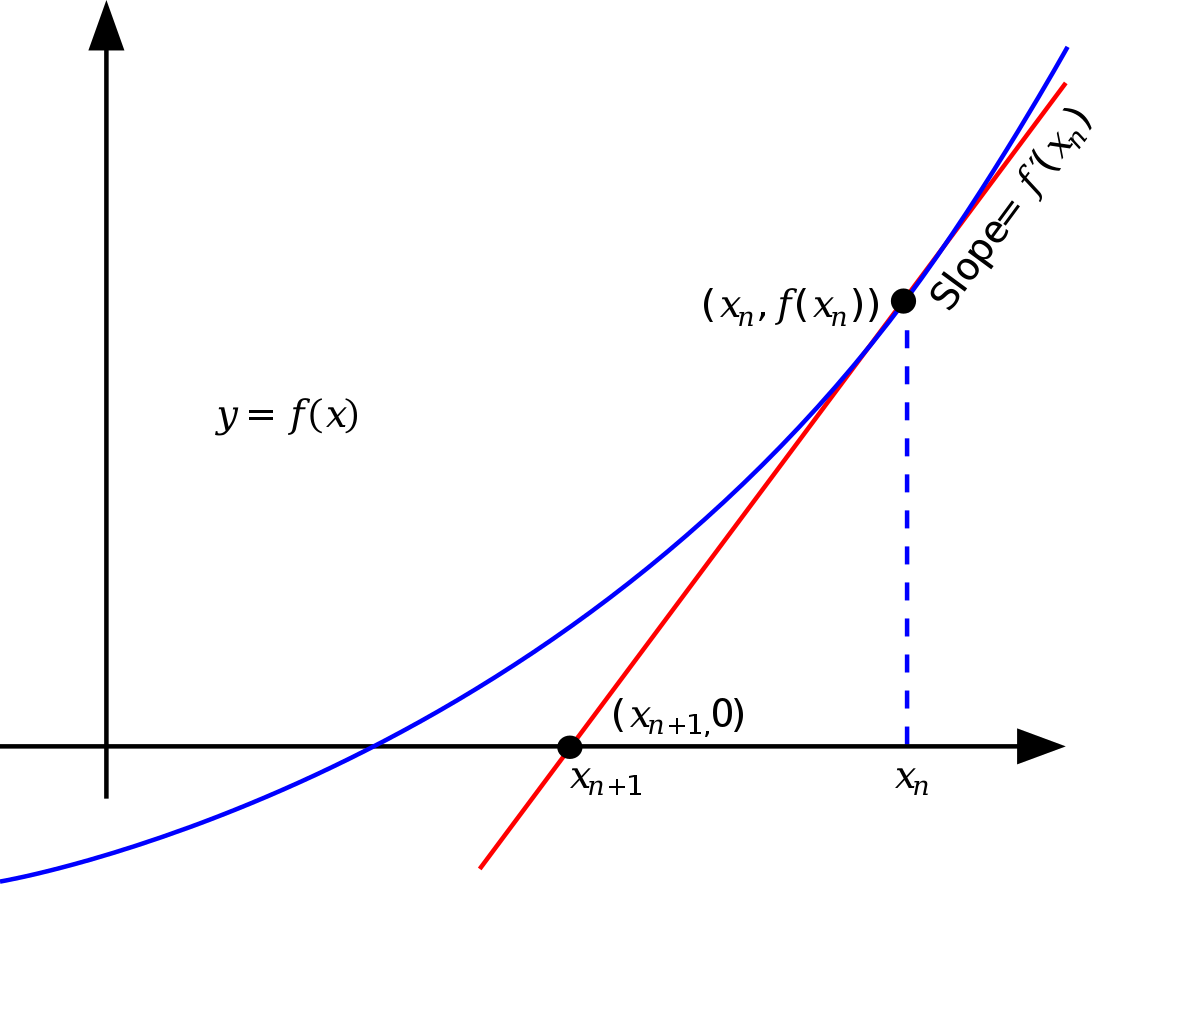
\includegraphics[width=0.75\textwidth]{plots/newtons_method.png}
	\caption{Veranschaulichung eines Iterationsschrittes des Newton-Verfahrens}
\end{figure}
\subsection*{Sekantenverfahren}
Für das Sekantenverfahren wählen wir zwei Anfangswerte $x_0,x_1 \in [0,1]$ und erhalten Näherungswerte durch
\[
	x_{n+1}= x_n - f(x_{n-1})\frac{x_{n-1}-x_{n-2}}{f(x_{n-1})-f(x_{n-2})}
\]
Es fällt sofort die Ähnlichkeit zum Newton-Verfahren auf, $f'$ wurde hier lediglich durch einen Differenzenquotienten ersetzt. Hier wählen wir also den Schnittpunkt der Sekanten durch $(x_{n-2}, f(x_{n-2}))$ und $(x_{n-1}, f(x_{n-1}))$ mit der $x$-Achse um den nächsten Näherungswert zu erhalten.
\begin{figure}[H]
	\centering
	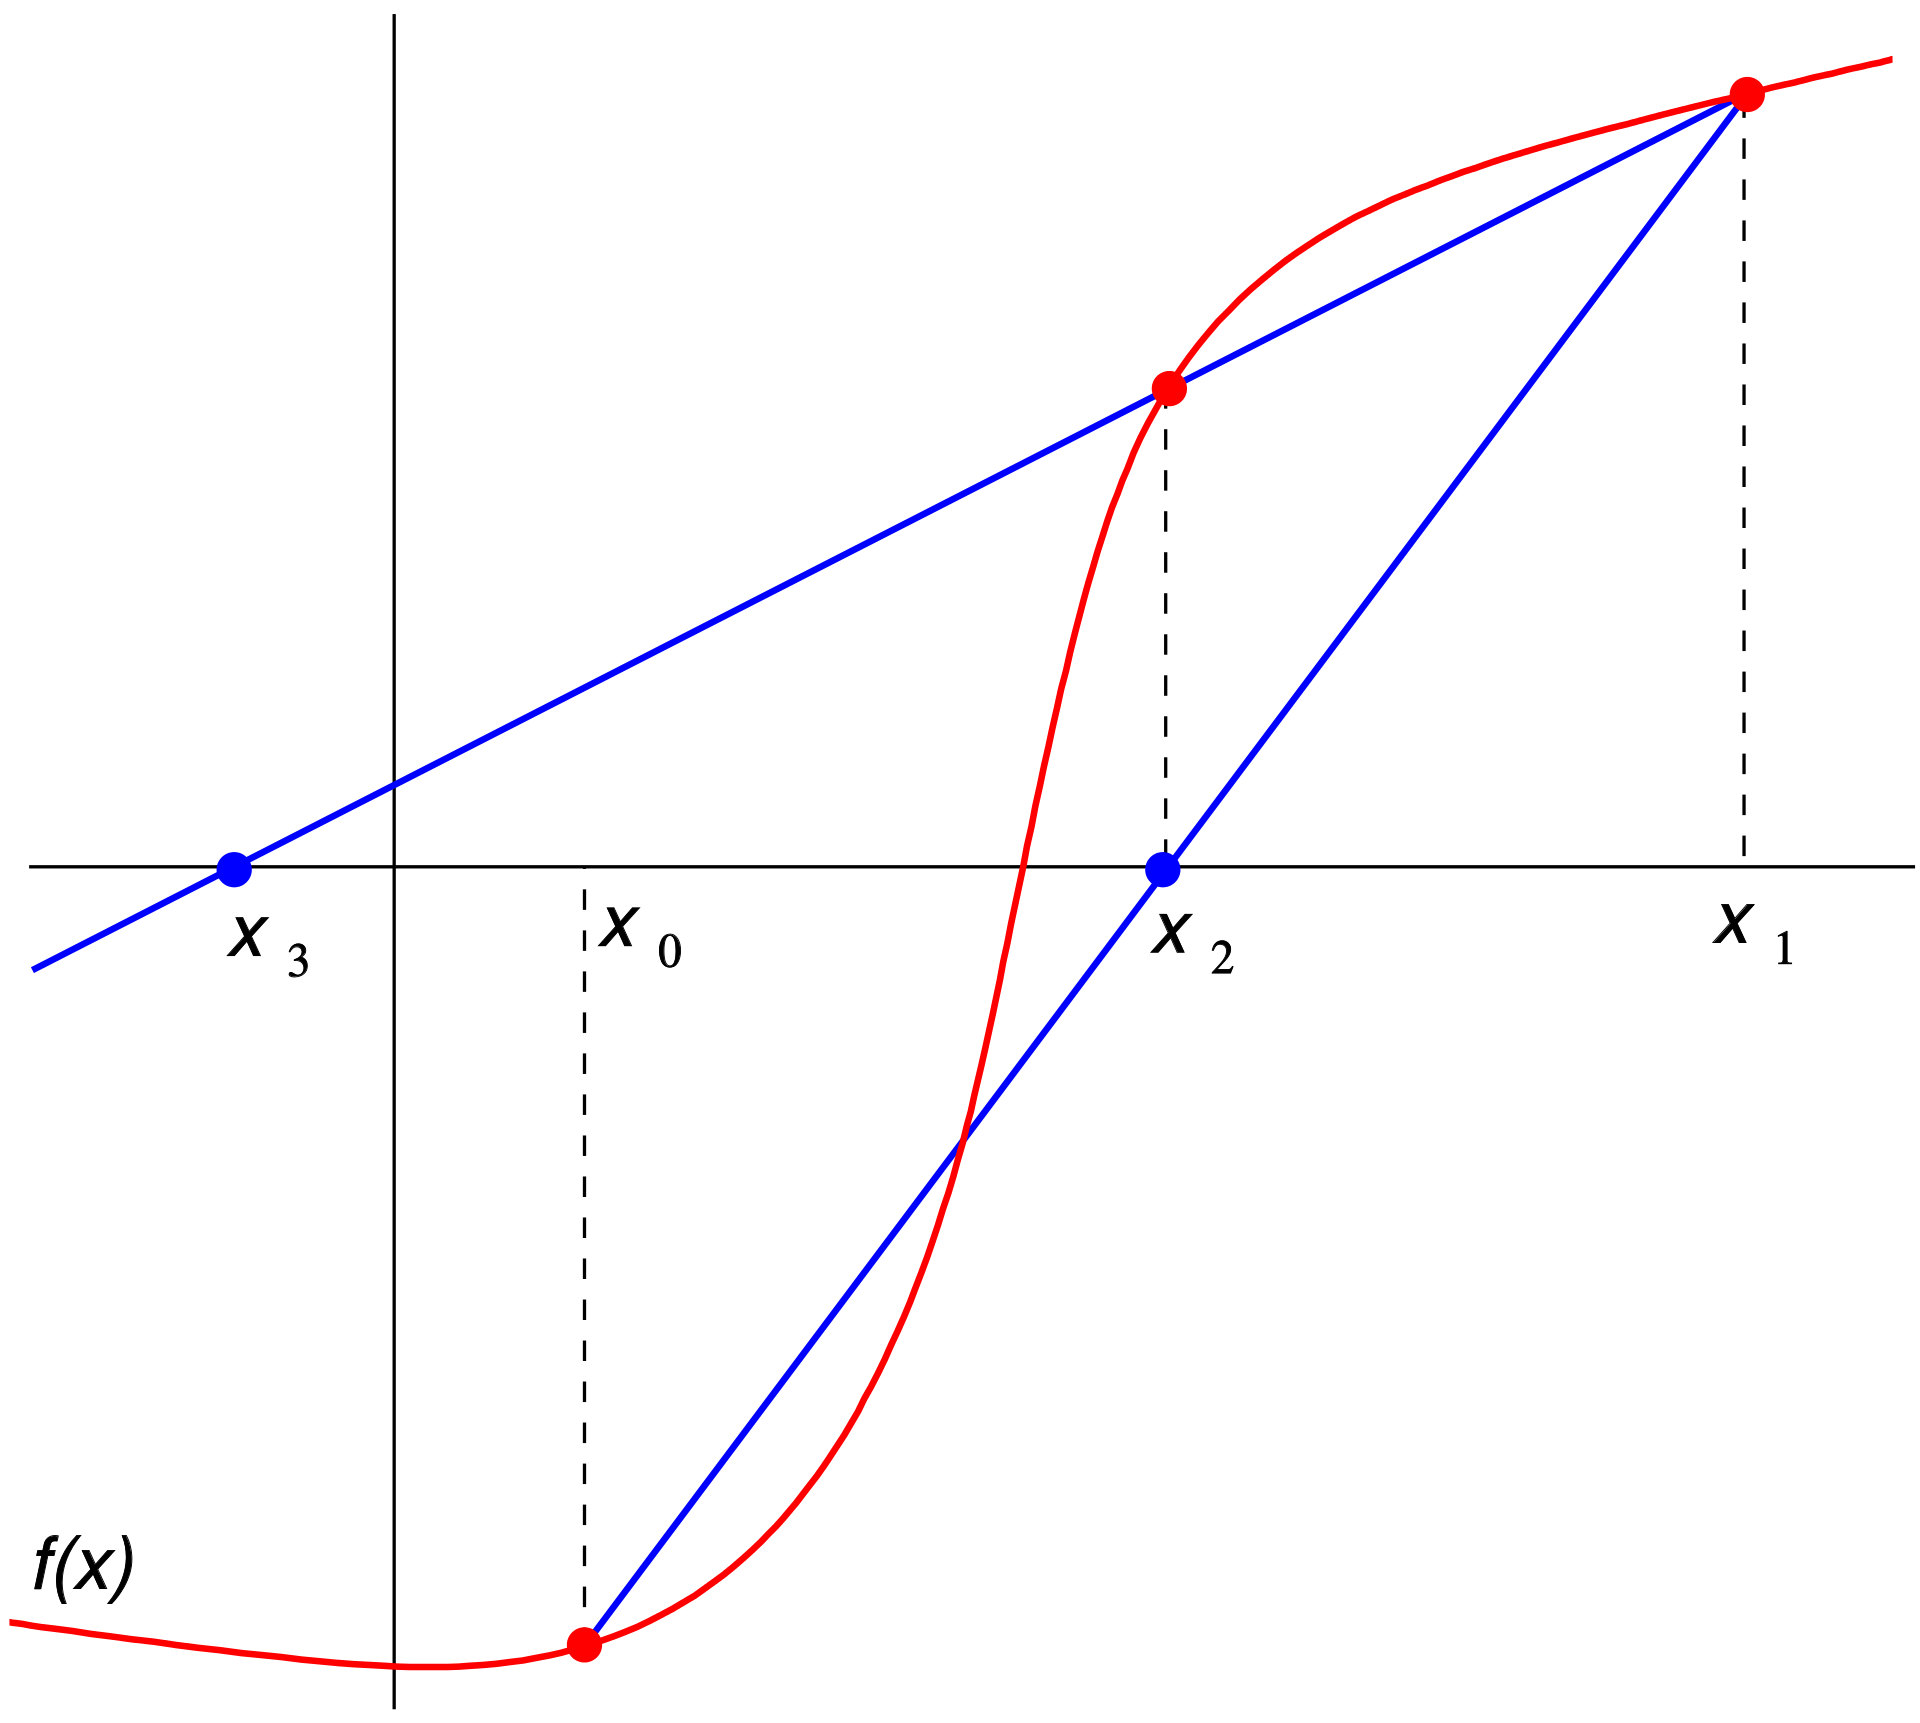
\includegraphics[width=0.75\textwidth]{plots/sekant.png}
	\caption{Veranschaulichung einiger Iterationsschritte des Sekantenverfahrens}
\end{figure}
\subsection*{Bisektionsverfahren}
Beim Bisektionsverfahren beginnen wir mit einem Startintervall $[a_0, b_0] \subseteq [0,1]$ mit $f(a_0)f(b_0) < 0$ (d.h. in diesem Intervall existiert eine Nullstelle). Wir betrachten in jedm Iterationsschritt nun den Mittelpunkt dieses Intervalles $x_n = \frac{a_n + b_n}{2}$, nun Überprüfen wir das Vorzeichen von $f, sgn(f(x_n))$ an dieser Stelle und Verkleinern das Intervall nach folgender Vorschrift:
\[
	a_{n+1} = \begin{cases}
		x_n\text{ falls } sgn(f(x_n))=sgn(f(a_n)), \\
		a_n\text{ sonst}
	\end{cases}, b_{n+1} = \begin{cases}
		x_n\text{ falls } sgn(f(x_n))=sgn(f(b_n)), \\
		b_n\text{ sonst}
	\end{cases}
\]
Dem informatikaffinen Leser fällt vielleicht die ähnlichkeit zur binären Suche auf.
\begin{figure}[H]
	\centering
	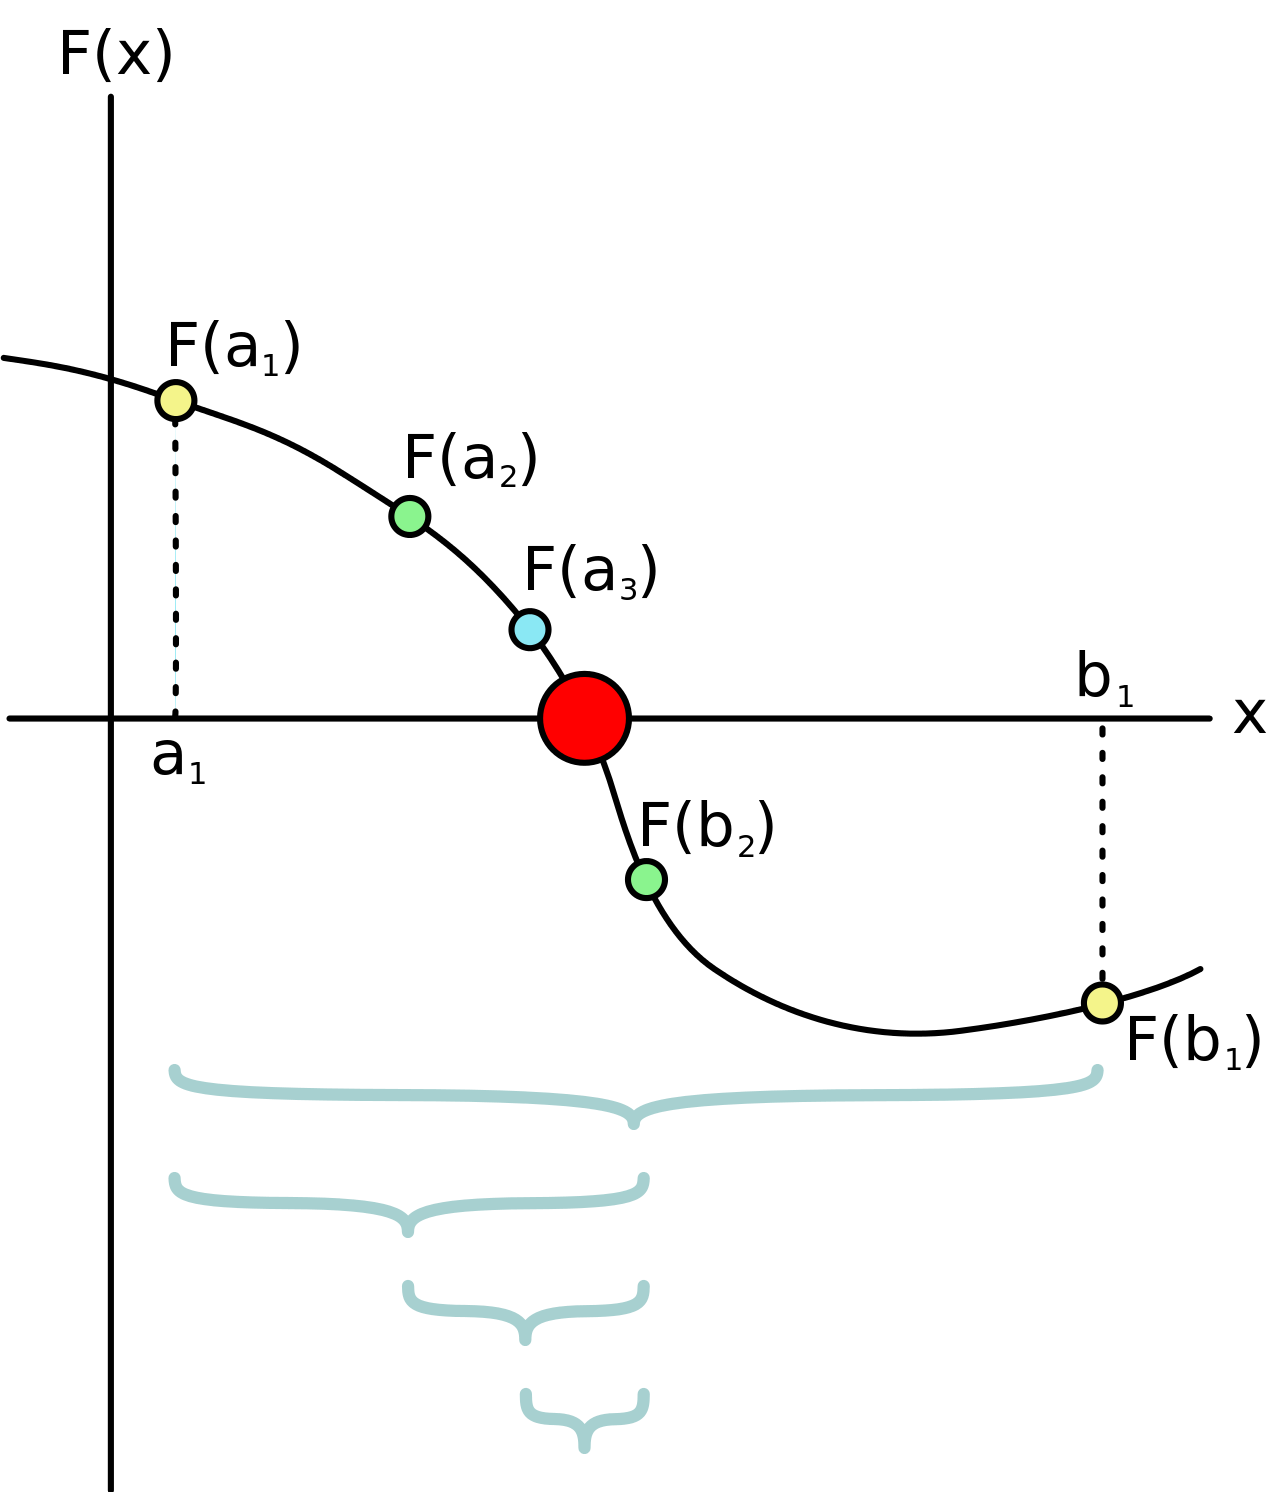
\includegraphics[width=0.75\textwidth]{plots/Bisection_method.png}
	\caption{Veranschaulichung einiger Iterationsschritte des Bisektionsverfahrens}
\end{figure}
\subsection*{Fixpunktverfahren}
Das Fixpunktverfahren sucht im Gegensatz zu den bisher erwähnten Algorithmen eine Lösung der Gleichung $g(x)=x$. Daher muss erst $f(x)=0$ entsprechend umgeformt werden. Anschliessend wählen wir einen Anfangswert $x_0\in[0,1]$ und wenden wiederholt $g$ darauf an:
\[
	x_{n+1}=g(x_n)
\]

\newpage
\section*{Diagramme}
\subsection*{Benötigte Iterationen}
Wir wollen zuerst die benötigten Iterationen der einzelnen Verfahren Gegenüberstellen. Wir wählten als Toleranzgrenze 0.00001, für Verfahren mit einem Benötigtem Startwert, wurde zur Nullstelle $x'$ der Startwert $x'-0.5$ gewählt. Für Verfahren mit zwei Startwerten $x'-0.2$ und $x'+0.3$. Die Wahl der Startwerte mag willkürlich erscheinen, der Trend der in den präsentierten Diagrammen zu erkennen ist deckt sich jedoch mit unseren Ergebnissen für andere Startwerte. Es wurde jeweils die Funktion $g_*$ gewählt mit der das Fixpunktverfahren tatsächlich ein Ergebnis liefert (mehr dazu im Vergleich der Verfahren).

\begin{figure}[H]
	\centering
	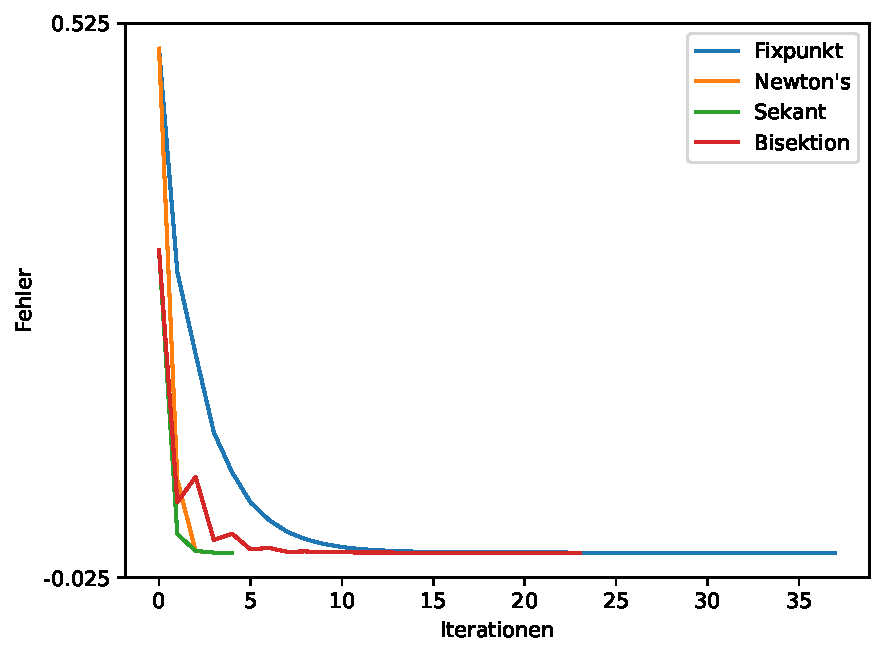
\includegraphics[width=0.75\textwidth]{plots/error_series_plot.pdf}
	\caption{$f_1(x) = x + e^x-2, g_{1,b}(x)=\log(2-x)$}
\end{figure}

\begin{figure}[H]
	\centering
	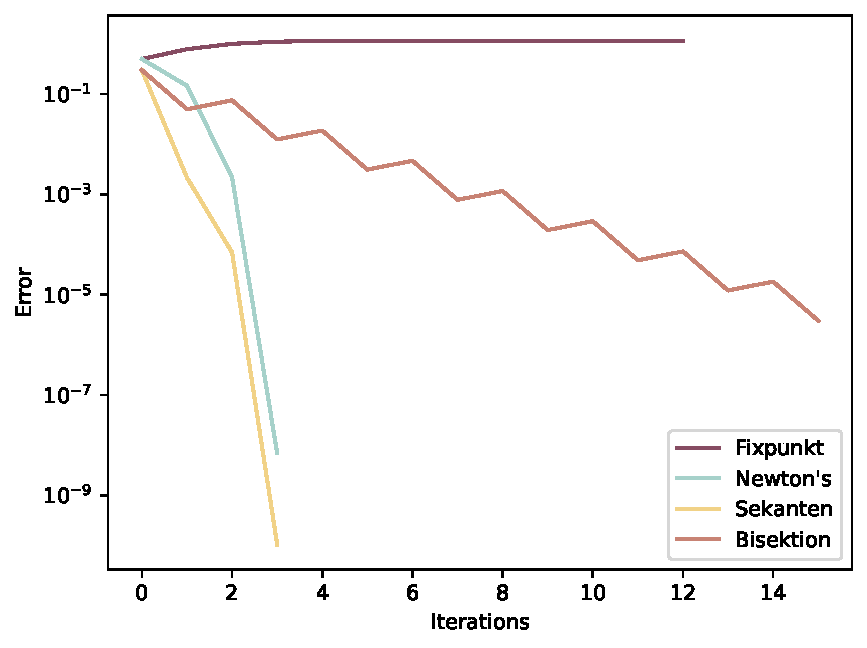
\includegraphics[width=0.75\textwidth]{plots/error_series_plot(1).pdf}
	\caption{$f_2(x) = 2x - \tan(x), g_{2,b}(x)=\arctan(2x)$}
\end{figure}

In Abb. 5 kann beobachtet werden, dass das Fixpunktverfahren gegen eine andere Nullstelle konvergiert als die anderen Verfahren. Wir konnten keinen Startwert finden, für den alle Verfahren gegen $0$ konvergieren.

\begin{figure}[H]
	\centering
	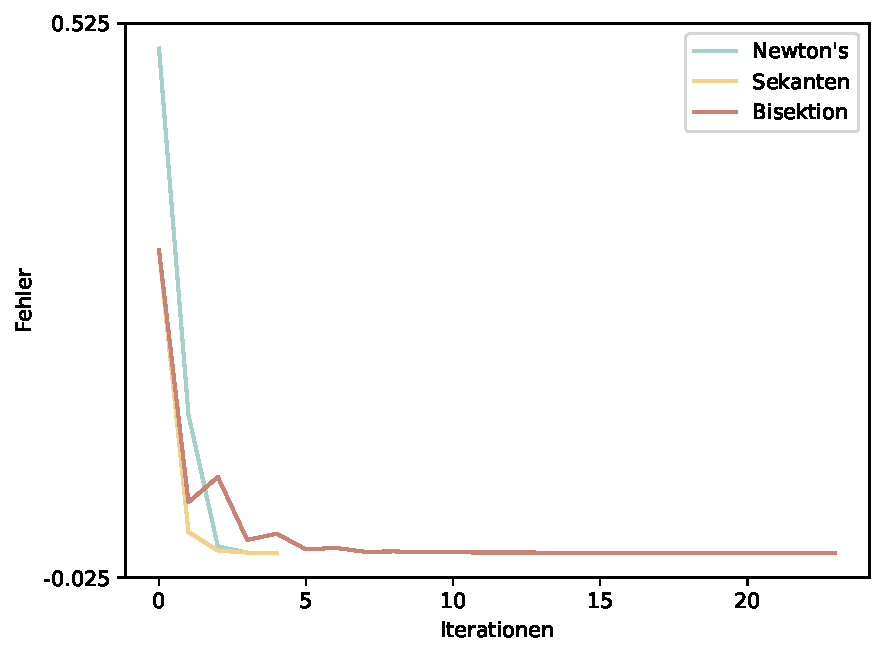
\includegraphics[width=0.75\textwidth]{plots/error_series_plot(2).pdf}
	\caption{$f_{3,2}(x) = -2x^2 + 4$}
\end{figure}


\begin{figure}[H]
	\centering
	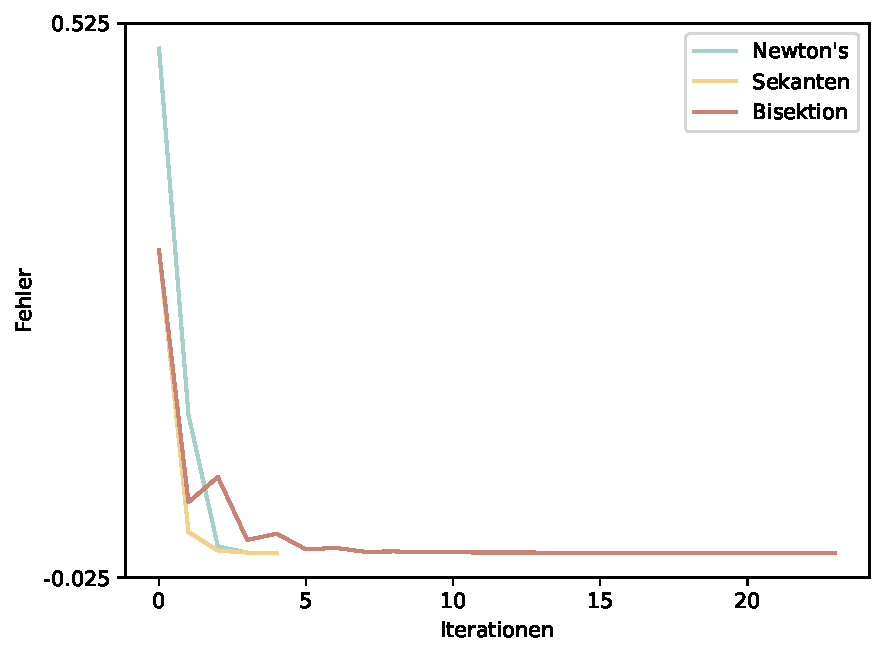
\includegraphics[width=0.75\textwidth]{plots/error_series_plot(3).pdf}
	\caption{$f_{3,1}(x) = -x^2 + 2$}
\end{figure}
\begin{figure}[H]
	\centering
	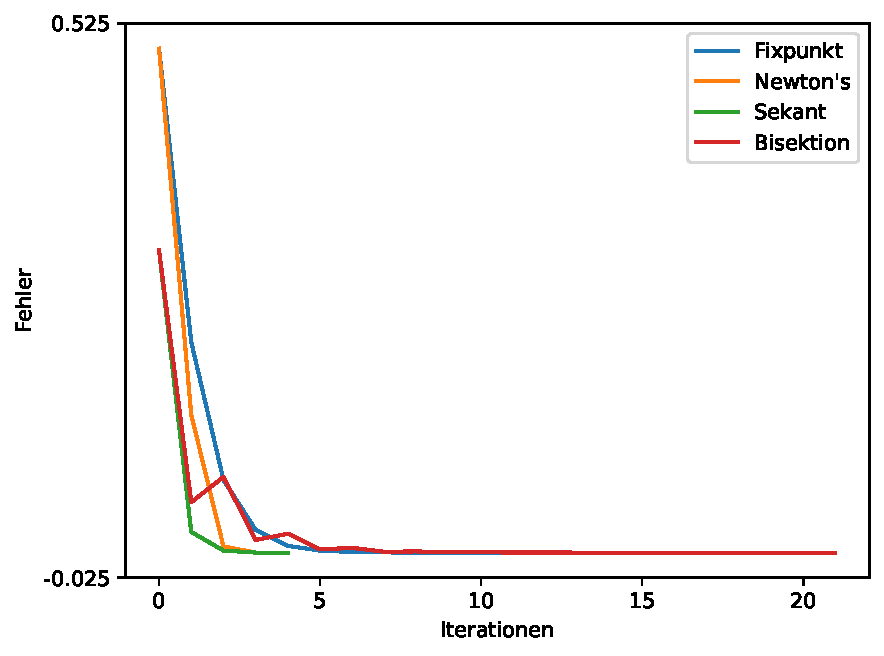
\includegraphics[width=0.75\textwidth]{plots/error_series_plot(4).pdf}
	\caption{$f_{3,\frac{1}{4}}(x) = -\frac{1}{4}x^2 +\frac{1}{2},  g_{3,\frac{1}{4}}(x)=-\frac{1}{4}x^2 + x + \frac{1}{2}$}
\end{figure}
In Abbildungen 7 und 8 ist insbesondere zu sehen, dass das Fixpunktverfahren divergiert.

\newpage
\subsection*{Variation der Startwerte}
Nun wollen wir noch gesondert betrachten, wie sich die Variation der Startwerte auf die benötigte Iterationen der einzelnen Verfahren auswirkt. Wir untersuchten die Funktion $f_1(x)=x+e^x-2$ beziehungsweise $g_{1,b}(x)=log(2-x)$, als Toleranzwert wurde immer 0.00001 gewählt.
\subsubsection*{Newton-Verfahren}
Das folgende Diagramm zeigt die vom Newton-Verfahren benötigten Iterationen um eine akzeptable Näherungslösung zu finden, aufgetragen gegen den gewählten Startpunkt.
\begin{figure}[H]
	\centering
	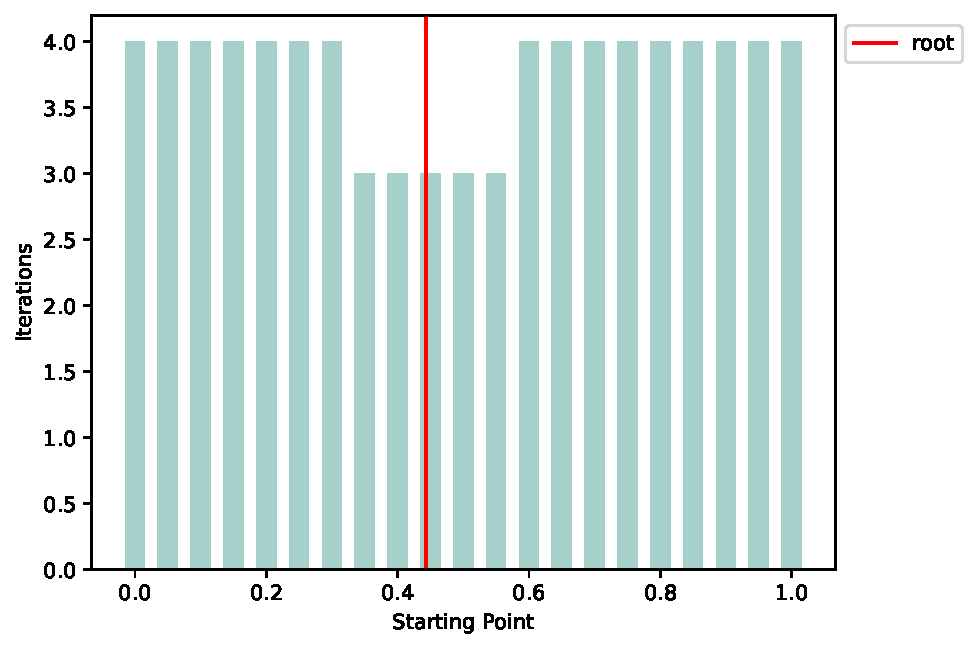
\includegraphics[width=0.75\textwidth]{plots/newton_iterations_by_starting_point.pdf}
\end{figure}
Es ist klar zu erkennen, dass das Verfahren schneller beendet ist, je näher der Startwert an der gesuchten Nullstelle liegt.
\subsubsection*{Sekantenverfahren}
Als erstes untersuchen wir, wie sich die benötigten Iterationen Verhalten wenn der Mittelpunkt der beiden Startwerte $x_0$ und $x_1$ verändert wird, wir diese Punkte derart, dass immer $x_1-x_0=\frac{1}{20}$
\begin{figure}[H]
	\centering
	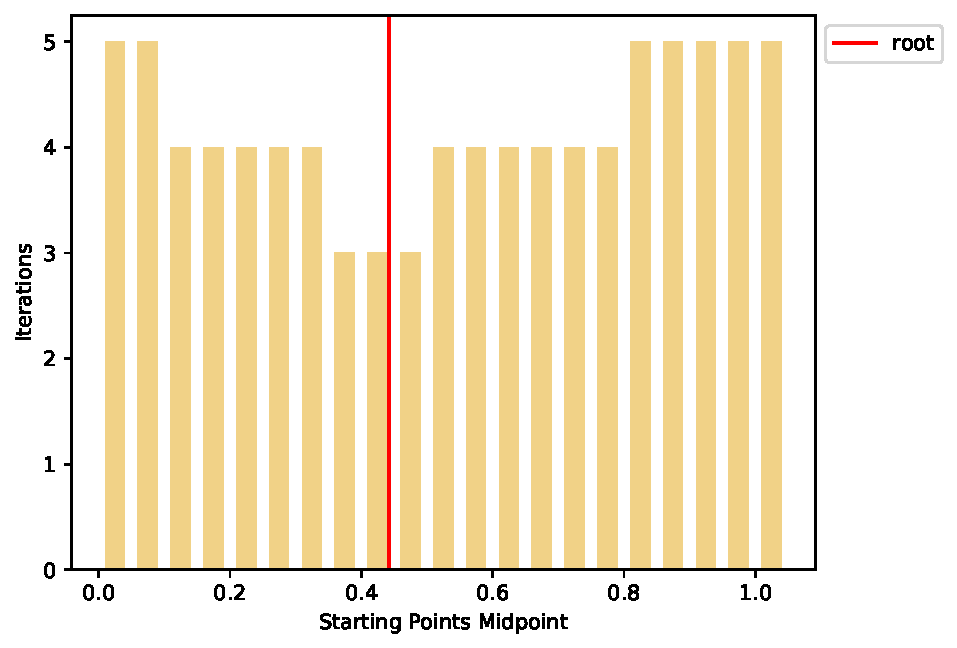
\includegraphics[width=0.75\textwidth]{plots/secant_iterations_by_midpoint_of_starting_points.pdf}
\end{figure}
Die benötigten Iterationen sind niedriger je näher der Mittelpunkt der beiden Startwerte an der gesuchten Nullstelle liegt.
Weiterhin betrachteten wir wie sich der Abstand von $x_0$ und $x_1$ auf die benötigten Iterationen auswirkt. Der Mittelpunkt der Anfagswerte liegt im folgendem Diagramm stets bei $0.5$
\begin{figure}[H]
	\centering
	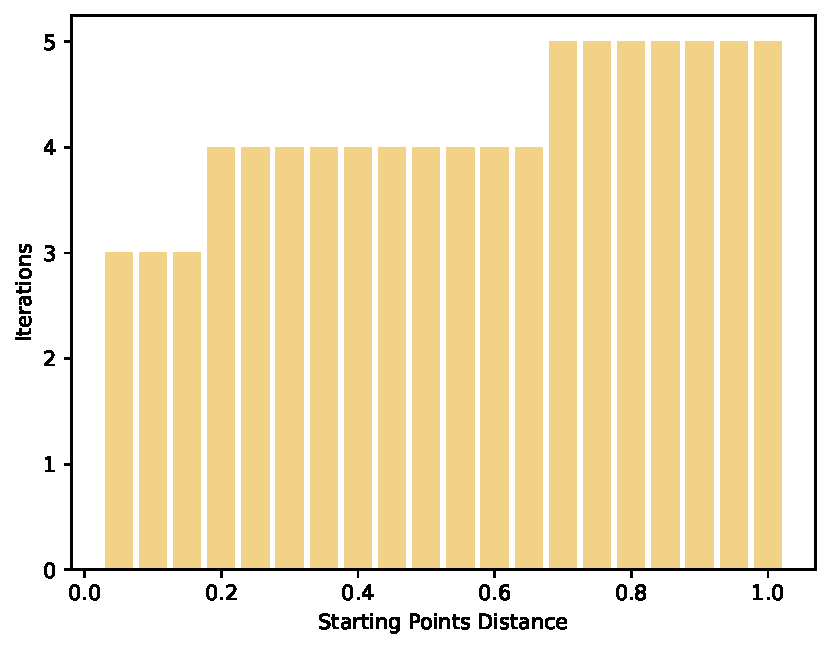
\includegraphics[width=0.75\textwidth]{plots/secant_iterations_by_starting_points_distance.pdf}
\end{figure}
Wir können erkennen, dass die benötigten Iterationen mit steigendem Abstand größer werden.
\subsubsection*{Bisektionsverfahren}
Zuerst betrachten wir wie sich die Größe des Startintervalls $[a_0, b_0]$ auf die benötigten Iterationen des Bisektionsverfahrens auswirkt. Das Intervall wurde hier stets so gewählt, dass die Nullstelle $x'$ eine Distanz von $1/80$ dazu hat.
\begin{figure}[H]
	\centering
	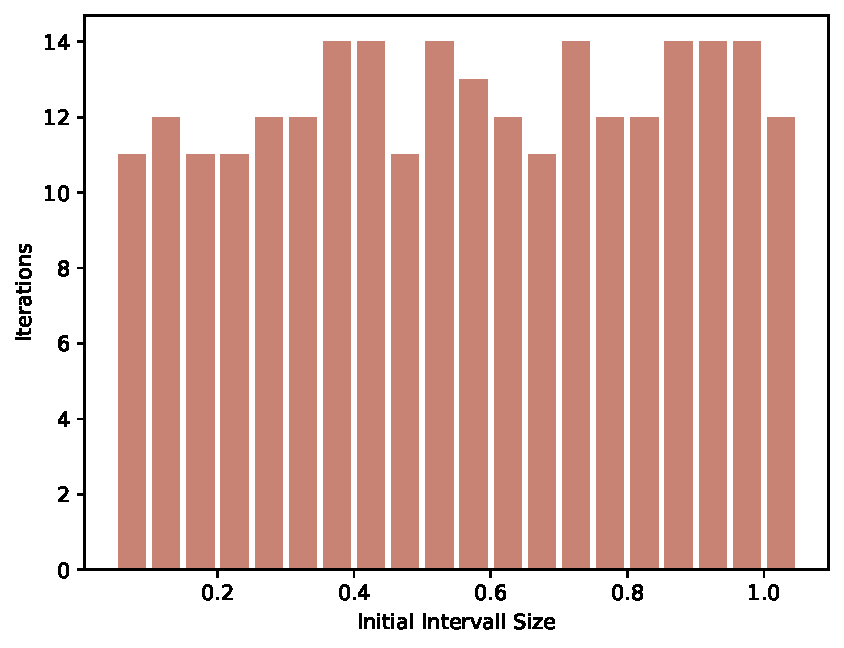
\includegraphics[width=0.75\textwidth]{plots/bisection_iterations_by_intervall_size.pdf}
\end{figure}
Es ist keine Offensichtliche Relation zwischen diesen Größen zu erkennen. Anschliessend untersuchen wir, wie sich die relative Position der gesuchten Nullstelle innerhalb des Intervalles auf die benötigten Iterationen auswirkt, das Startintervall hat hier immer die Größe 1.
\begin{figure}[H]
	\centering
	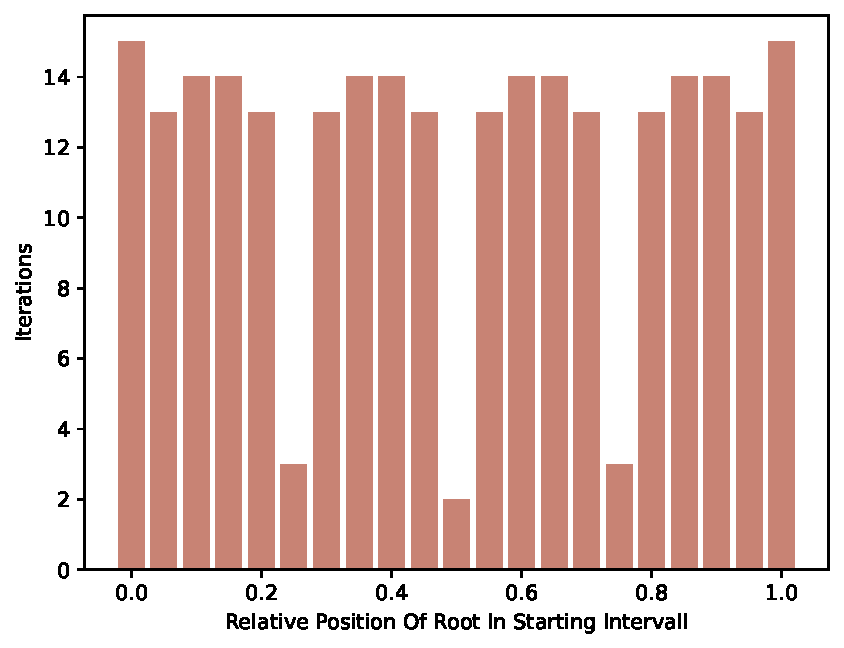
\includegraphics[width=0.75\textwidth]{plots/bisection_iterations_by_relative_position_of_root.pdf}
\end{figure}
Wir erkennen, dass an gewissen Positionen die benötigten Iterationen dramatisch sinken. Diese Positionen sind in der Nähe von $\frac{1}{4}, \frac{1}{2}$ und $\frac{3}{4}$; also Stellen, die nach sehr wenigen Iterationen Mittelpunkt des Intervalls sind.
\subsubsection*{Fixpunktverfahren}
Wir untersuchen auch hier die Beziehung zwischen Startpunkt und benötigten Iterationen.
\begin{figure}[H]
	\centering
	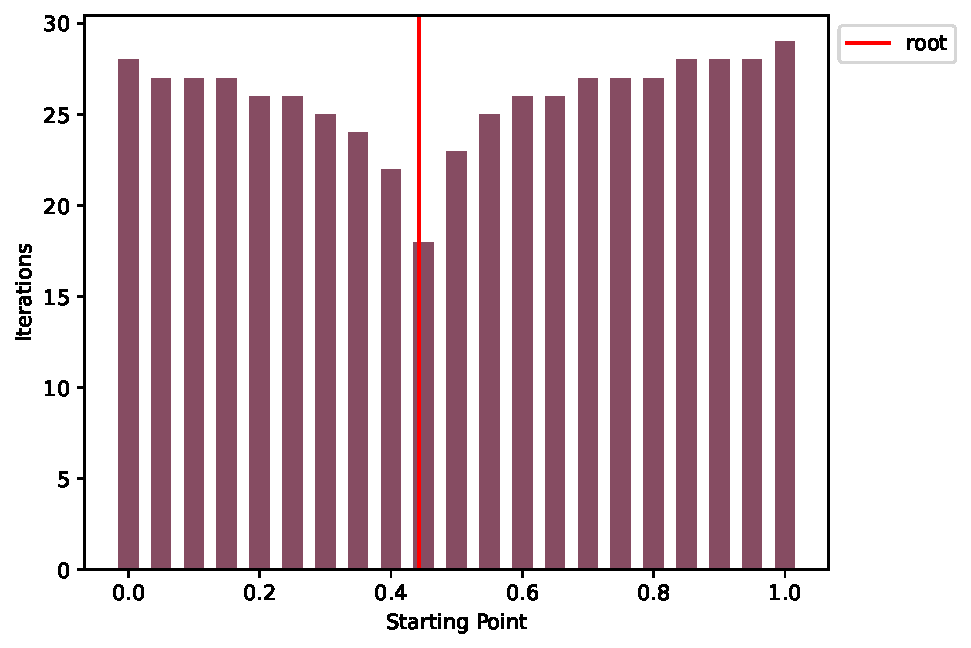
\includegraphics[width=0.75\textwidth]{plots/fixed_point_iterations_by_starting_point.pdf}
\end{figure}
Wieder können wir erkennen, dass weniger Iterationen benötigt werden, je näher der Startpunkt an der Nullstelle liegt.
\section*{Vergleich der Verfahren}
In unseren Experimenten, ist das Newton Verfahren im Durchschnitt am Performantesten und relativ insensitiv gegenüber der Wahl des Startwertes. Allerdings ist zu beachten, dass bei diesem Verfahren die Ableitung der Betrachteten Funktion benötigt wird, will man daher eine "vollautomatische" Version nutzen, muss zusätzlich noch algorithmisch differenziert werden. Am zweit besten schneidet das Sekantenverfahren ab, der geringe unterschied der benötigten Iterationen im Vergleich zum Newton Verfahren, könnte dadurch ausgeglichen werden, dass hier kein kompliziertes automatisches Differenzieren implementiert werden muss. Bei beiden Algorithmen besteht die Möglichkeit, dass ein Abbruch nötig ist, da bei entsprechender Steigung eine Division durch 0 ausgeführt wird. Das Bisektionsverfahren benötigt durchschnittlich wesentlich mehr Iterationen als die beiden bisher genannten Verfahren. Ein weiterer Nachteil ist, dass schon vor der Anwendung des Verfahrens ungefähr bekannt sein muss wo alle Nullstellen der Untersuchten Funktion liegen, da im Startintervall nur eine Nullstelle liegen darf. Am schlechtesten schneidet das Fixpunktverfahren ab, abgesehen davon ist es am problematischsten, dass für die Anwendung die untersuchte Funktion erst korrekt umgeformt werden muss. Mit korrekt ist hier gemeint, dass für viele Umformungen das Fixpunkverfahren divergiert (Beispielsweise $g_{1,a}$ oder $g_{2,a}$). Eine hinreichende bedingung für die Konvergenz des Fixpunktverfahrens liefert der Banachsche Fixpunktsatz, d.h. für die Umformung $g$ von $f$ sollte gelten $|g'| < 1$. Jedoch kann es selbst bei geigneten Umformungen zu komplikationen kommen, In Abbildung 5 ist zu sehen, dass das Fixpunktverfahren gegen eine andere Nullstelle als die anderen Verfahren konvergiert, tatsächlich fanden wir keinen Startwert mit dem das Fixpunktverfahren die gewünschte Nullstelle liefert.

\end{document}